%%%%%%%%%%%%%%%%%%%%%%%%%%%%%%%%%%%%%%%%%
% Short Sectioned Assignment
% LaTeX Template
% Version 1.0 (5/5/12)
%
% This template has been downloaded from:
% http://www.LaTeXTemplates.com
%
% Original author:
% Frits Wenneker (http://www.howtotex.com)
%
% License:
% CC BY-NC-SA 3.0 (http://creativecommons.org/licenses/by-nc-sa/3.0/)
%
%%%%%%%%%%%%%%%%%%%%%%%%%%%%%%%%%%%%%%%%%

%----------------------------------------------------------------------------------------
%	PACKAGES AND OTHER DOCUMENT CONFIGURATIONS
%----------------------------------------------------------------------------------------

\documentclass[paper=a4, fontsize=11pt]{scrartcl} % A4 paper and 11pt font size

\usepackage[T1]{fontenc} % Use 8-bit encoding that has 256 glyphs
\usepackage{fourier} % Use the Adobe Utopia font for the document - comment this line to return to the LaTeX default
\usepackage[english]{babel} % English language/hyphenation
\usepackage{amsmath,amsfonts,amsthm} % Math packages
\usepackage[utf8]{inputenc}
\usepackage{lipsum} % Used for inserting dummy 'Lorem ipsum' text into the template
\usepackage{xcolor}
\usepackage{graphicx}


\usepackage{listings}
  \usepackage{courier}
 \lstset{
         basicstyle=\footnotesize\ttfamily, % Standardschrift
         %numbers=left,               % Ort der Zeilennummern
         numberstyle=\tiny,          % Stil der Zeilennummern
         %stepnumber=2,               % Abstand zwischen den Zeilennummern
         numbersep=5pt,              % Abstand der Nummern zum Text
         tabsize=2,                  % Groesse von Tabs
         extendedchars=true,         %
         breaklines=true,            % Zeilen werden Umgebrochen
         keywordstyle=\color{red},
    		frame=b,         
 %        keywordstyle=[1]\textbf,    % Stil der Keywords
 %        keywordstyle=[2]\textbf,    %
 %        keywordstyle=[3]\textbf,    %
 %        keywordstyle=[4]\textbf,   \sqrt{\sqrt{}} %
         stringstyle=\color{white}\ttfamily, % Farbe der String
         showspaces=false,           % Leerzeichen anzeigen ?
         showtabs=false,             % Tabs anzeigen ?
         xleftmargin=17pt,
         framexleftmargin=17pt,
         framexrightmargin=5pt,
         framexbottommargin=4pt,
         %backgroundcolor=\color{lightgray},
         showstringspaces=false      % Leerzeichen in Strings anzeigen ?        
 }
 \lstloadlanguages{% Check Dokumentation for further languages ...
         %[Visual]Basic
         %Pascal
         %C
         %C++
         %XML
         %HTML
         Java
 }
    %\DeclareCaptionFont{blue}{\color{blue}} 

  %\captionsetup[lstlisting]{singlelinecheck=false, labelfont={blue}, textfont={blue}}
  \usepackage{caption}
\DeclareCaptionFont{white}{\color{white}}
\DeclareCaptionFormat{listing}{\colorbox[cmyk]{0.43, 0.35, 0.35,0.01}{\parbox{\textwidth}{\hspace{15pt}#1#2#3}}}
\captionsetup[lstlisting]{format=listing,labelfont=white,textfont=white, singlelinecheck=false, margin=0pt, font={bf,footnotesize}}


\usepackage{sectsty} % Allows customizing section commands
\allsectionsfont{\centering \normalfont\scshape} % Make all sections centered, the default font and small caps

\usepackage{fancyhdr} % Custom headers and footers
\pagestyle{fancyplain} % Makes all pages in the document conform to the custom headers and footers
\fancyhead{} % No page header - if you want one, create it in the same way as the footers below
\fancyfoot[L]{} % Empty left footer
\fancyfoot[C]{} % Empty center footer
\fancyfoot[R]{\thepage} % Page numbering for right footer
\renewcommand{\headrulewidth}{0pt} % Remove header underlines
\renewcommand{\footrulewidth}{0pt} % Remove footer underlines
\setlength{\headheight}{13.6pt} % Customize the height of the header

\numberwithin{equation}{section} % Number equations within sections (i.e. 1.1, 1.2, 2.1, 2.2 instead of 1, 2, 3, 4)
\numberwithin{figure}{section} % Number figures within sections (i.e. 1.1, 1.2, 2.1, 2.2 instead of 1, 2, 3, 4)
\numberwithin{table}{section} % Number tables within sections (i.e. 1.1, 1.2, 2.1, 2.2 instead of 1, 2, 3, 4)

\setlength\parindent{0pt} % Removes all indentation from paragraphs - comment this line for an assignment with lots of text

%----------------------------------------------------------------------------------------
%	TITLE SECTION
%----------------------------------------------------------------------------------------

\newcommand{\horrule}[1]{\rule{\linewidth}{#1}} % Create horizontal rule command with 1 argument of height

\title{	
\normalfont \normalsize 
\textsc{ENSEIRB-MATMECA} \\ [25pt] % Your university, school and/or department name(s)
\horrule{0.5pt} \\[0.4cm] % Thin top horizontal rule
\huge Accélérateurs de calculs \\ % The assignment title
\horrule{2pt} \\[0.5cm] % Thick bottom horizontal rule
}

\author{Caneill Pierre-Yves, Lux Benjamin} % Your name

\date{\normalsize\today} % Today's date or a custom date

\begin{document}

\maketitle % Print the title

%----------------------------------------------------------------------------------------
%	Version 1
%----------------------------------------------------------------------------------------

\section{Multiplication de matrices}
Nous avons réalisé cette partie en \verb!CUDA!.
\subsection{Version Simple}
Le premier kernel est très simple, chaque thread de calcul va se
charger de calculer sa case de la matrice.

Bien que cette version soit très simple on arrive à obtenir des
résultats bien plus interessant que sur CPU.

\subsection{Optimisation mémoire}
La deuxième version va esseyer d'optimiser les accès mémoire en
travaillant par rangée. Ainsi les différents wrap accèderont à des
données proches.

\subsection{Optimisation par blocs}
Enfin la dernière optimisation que nous avons fait était de faire des
calculs matriciels par blocs. Afin de réutiliser la mémoire. Pour cela
nous avons chargé en mémoire partagée le bloc de travail pour ensuite
faire les calculs.

\begin{lstlisting}
__global__ void matrixMul3(float * g_C, float * g_A, float *g_B,int wa, int wb){
  const int TILE_WIDTH = 16;
  int tx = threadIdx.x;
  int ty = threadIdx.y;
  int bx = blockIdx.x;
  int by = blockIdx.y;

  __shared__ float s_a[TILE_WIDTH][TILE_WIDTH];
  __shared__ float s_b[TILE_WIDTH][TILE_WIDTH];

  int row = bx*blockDim.y + tx;
  int col = by*blockDim.x + ty;
  float result = 0;

  int i = 0;
  for(i = 0; i < wa/TILE_WIDTH; ++i){
    s_a[tx][ty] = g_A[i*TILE_WIDTH + row*wa +ty];
    s_b[tx][ty] = g_B[(i*TILE_WIDTH*wa)+tx*wa+ col];
    __syncthreads();

    int k =0;
    for(k=0;k<TILE_WIDTH;++k){
      result += s_a[tx][k] * s_b[k][ty];
    }
    __syncthreads();
  }

  g_C[row*wa+col] = result;

}
\end{lstlisting}


\subsection{Comparaison des différentes versions}
Nous avons implémenté une version sur le processeur en utilisant
openMP.

Le premier graphique présente les différentes version GPU avec la
version CPU. On observe que la version CPU prend énormément plus de
temps que les différentes version GPU.
\begin{figure}[!h]
  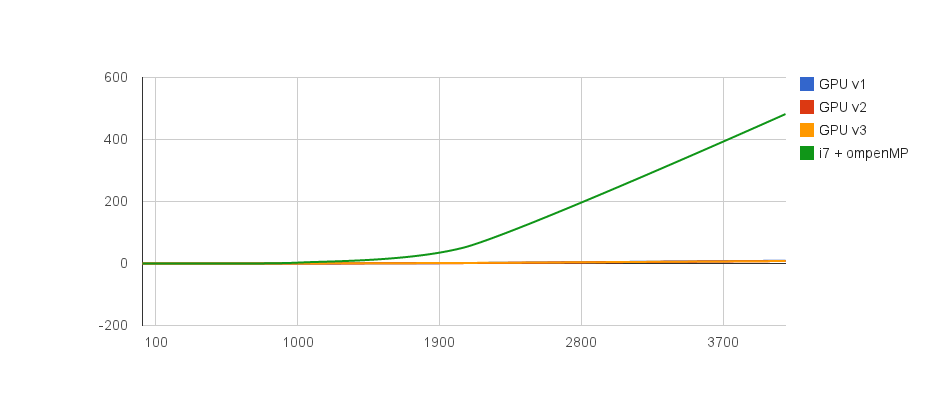
\includegraphics[width=1\textwidth]{chart_1.png}
  \centering
  \caption{Comparaison GPU / CPU}
\end{figure}

Le deuxième graphique présente une comparaison des différentes
versions GPU entre elles. On voit que elles sont dans le même ordre de
grandeur. On a été assez surpris que la version par blocs n'aille pas
significativement plus vite que les autres. S'est peut être lié à une
erreur d'implémentation.

\begin{figure}[!h]
  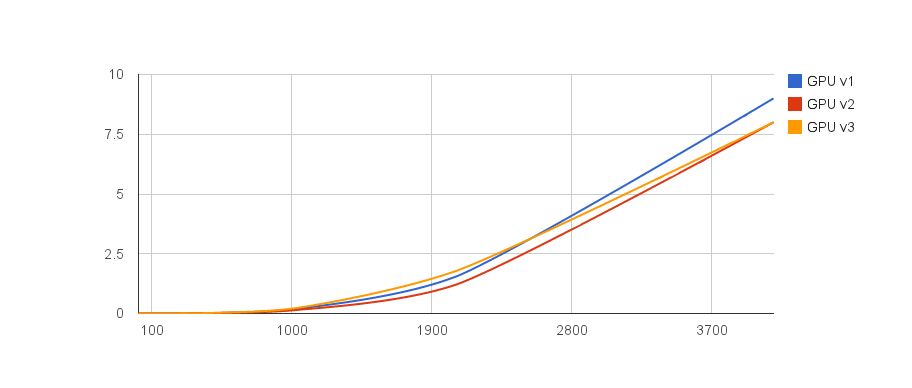
\includegraphics[width=1\textwidth]{chart_2.png}
  \centering
  \caption{Comparaison GPU}
\end{figure}

\subsection{Sortie du programme}
\begin{verbatim}
System Informations
-------------------

Number of devices : 1
Device Informations
  Name : GeForce GT 555M
  Memory : 2147155968
  WarpSize : 32
  Max Threads Per Block : 1024
  Multi processor count : 3


Multiplication with CPU using openMP
-----------------------------------

Size Matrix 2048x2048
Starting multiplication CPU ...[OK]
Time : 47.579655 s
Mflop/s : 361.075951 


Multiplication without optimisation
-----------------------------------

Size Matrix 2048x2048

Starting multiplication GPU ...[OK]
Time : 1.525846 s
Mflop/s : 11259.256637 
Multiplication correct
Speed UP x30


Multiplication with first optimisation
-----------------------------------------

Size Matrix 2048x2048
Starting multiplication GPU ...[OK]
Time : 1.198078 s
Mflop/s : 14339.536761 
Multiplication correct
Speed UP x39


Multiplication with second optimisation
-----------------------------------------

Size Matrix 2048x2048
Starting multiplication GPU ...[OK]
Time : 1.761853 s
Multiplication correct
Speed UP x26
\end{verbatim}


\section{Factorisation de Cholesky}

Cette seconde partie à était faite en \textit{OpenCl}.

\subsection{Présentation générale de l'algorithme}
La factorisation de cholesky d'une matrice $A$, pour les matrices
carrées symétriques définies positives, permet de trouver une matrice
carrée triangulaire inférieure $L$ telle que $A\ =\ L\times L^{T}$. \\

Une fois cette décomposition effectuée, la résolution de l'équation
$A\times x\ =\ b$, devient un simple calcul "décente-remontée" en
$\Theta(n^2)$.

L'algorhitme de base est le suivant :
\begin{verbatim}
DEBUT
Pour i de à n                         (1)
  a[i,i] = sqrt(a[i,i])
  
  Pour j de i+1 à n                   (2)
    a[i,j] = a[i,j] / a[i,i]
  Pour j de i+1 à n                   (3)
    Pour k de i+1 à j                 (4)
      a[k,j] = a[k,j] - a[i,j]*a[i,j] 
FIN
\end{verbatim}

\subsection{Principe de base}
Les deux versions ont un corps commun.  On commence par allouer un
vecteur de $float$ en mémoire qui représentera la matrice $A$. On
l'initialise de sort à avoir un matrice respectant les conditions
initiales demandées. On crée ensuite un contexte OpenCL de type
$cl\_context$. On compile et charge le ou les kernel en mémoire
GPU/CPU. On charge en mémoire un $cl\_meme$ qui est un buffer
identique au buffeur de $A$. Les calculs sur ce buffer sont ensuite
effectué. On récuppère par recopie le résultat dans le buffer de $A$.
On vérifit ensuite les calculs en remplissant de zéro la partie
triangulaire strictement supérieur et multipliant la matrice ainsi
obtenue avec sa transposé. Cette matrice devrai être identique à la
matrice de départ et donc leur différence être nulle.


\subsection{Algorithme de base}
La première version implémentée de cette factorisation en
\textit{OpenCL} reprend basiquement l'algorithme précédent.Elle se
compose d'un seul kernel. Chacun thread du kernel représente un
élément de la matrice. Ici la mémoire locale n'est pas utilisée en
dehors de l'indice courant.  Le parallèlisme se fait sur les boucles
$(2)$ et $(4)$.  Puisque les synchronisations ne se font qu'au sein
d'un même Work Groupe on doit mettre tous les threads dans le même
Work Groupe. Du coup ici la distionction global/local ne sert pas.


\subsection{Algorithme par bloc}
Cette seconde version impélente un algorithme par bloc. Elle se
compose de trois kernel. Chacun est exécuté tour à tour sur la
même matrice. la boucle de calcul dans le code $C$ est alors :

\begin{verbatim}
DEBUT
Charger le buffer A en mémoire
Pour i de 1 à n/work_groupe_size faire
  Kernel_diagonal(A,i)
  Kernel_sous_diagonal(A,i)
  Kernel_inferieur_droit(A,i)

Recuperer le buffer A
FIN
\end{verbatim}

Il est à noter que chacun de ces kernel récupère en mémoire locale les
blocs nécessaires au calcul afin d'optimiser le temps de recherche des
éléments nécessaires aux calculs.

Par la suite les entiers consécutifs de $1$ à $n$ seront notés
$[|1;n|]$. Les blocs seront notés $B_{(i,j)}$, avec $(i,j)\in[|1;n|]$,
et $n = \frac{N}{worker\_groupe\_size}$


\paragraph{Kernel 1: diagonale}

Le premier kernel ne travail que sur le sous bloc diagonal. Il s'agit
en résumé d'éxécuter l'algorithme de Cholesky sur le bloc $B_{(i,i)}$.

\paragraph{Kernel 2: sous-diagonale} 

Le second kernel met à jour les blocs $B_{(i,j)}$, avec
$j\in[|i+1;n|]$. Il correspond à la boucle $(2)$ (et une petite partie
de la boucle $(3)$).  Les threads ont besoin des valeurs de leur blocs
local $B_{(i,j)}$ ainsi que des valeurs du bloc $B_{(i,i)}$. Même si
seule la première moitié de ce dernier bloc est nécessaire, autant
copier le bloc entier puisque les copies ce font en parrellèle, un
$if$ aurait surement même était plus coûteux.

Chaque colone du bloc $B_{(i,j)}$ est d'abord divisée par l'élément
diagonale correspondant, puis met à jour la partie droite restante du
bloc.

\paragraph{Kernel 3: inférieur droit} 

Le troisième kernel met à jour les blocs inférieurs droits, comprendre
ici les blocs $B_{(k,j)}$ avec $k\in[|i+1;n|]$ et $j\in[|k;n|]$. Pour
mettre à jour ce bloc les threads ont besoin de copier en local deux
blocs supplémentaires, $B_{i,k}$ et $B_{i,j}$. On se rend compte que
l'opération correspond à faire : $B_{k,j}\ =\ B_{k,j}\ -\ B_{i,k}
\times B_{i,j}^T$. Cette opération peut être implémentée comme :
$$B_{k,j}[x,y]\ =\ B_{k,j}[x,y]\ - \sum_{l=1}^{wg\_size}(B_{i,k}[l,y]
\times B_{i,j}[l,x])$$





\subsection{Résultats (Tests)}
puuut putputputput


\subsection{Performance}
No GPU, No perf.

\section{Questions}

\subsection{Question 2}
\subsection{Question 3}



























\end{document}



